All single-top uncertainties are derived by MC-to-MC comparison,  and split into the normalisation acceptance uncertainties and the 
shape uncertainties,  as described in Section~\ref{sec:systematics_backgroundmodelling}, 
following the  \href{https://twiki.cern.ch/twiki/bin/view/AtlasProtected/TopMCSystematicsR21}{\underline{recommendations of the Top modelling group}}. 

Uncertainties due to PDF, additional radiation (ISR) and FSR are evaluated using internal alternative weights present in all single-top nominal samples. 
Using the \texttt{PDF4LHC15\_30} PDF set, the uncertainties are estimated by combining the difference between the error sets and the nominal set following the recommendations in Ref.\cite{Butterworth:2015oua}.

Uncertainties from the parton shower, matrix element (ME) and single top interference ($Wt$-channel) are estimated using 
the differences between the nominal samples and the corresponding alternative samples, as reported in Table~\ref{sec:systs:tab:systematics_singletop}. 
As the $W$t-channel contribution dominates over the $t$-channel and $s$-channel contributions, only the contribution from the $Wt$-channel 
is considered. Parton shower and hadronisation uncertainties (PS) are evaluated comparing the AF2 nominal samples showered with Pythia8 
with alternative AF2 samples showered with Herwig7.  The ME NLO matching uncertainty is evaluated comparing  the AF2 nominal Powheg+Pythia8 
samples to the alternative AF2 aMcAtNlo+Pythia8 samples.  Uncertainty due single-top interference is evaluated comparing the full simulated nominal 
Powheg+Pythia8 samples with diagram removal (DR) scheme to the alternative full simulation Powheg+Pythia8 sample with diagram subtraction (DS) 
scheme.

\begin{table}
  \centering
  \begin{tabular}{|c|c|c|}
  \hline
  Source & DSID & Name\\
  \hline
  Nominal & 410646, 410647 &PowhegPythia8EvtGen\_A14\_Wt\_DR\_inclusive \\
  ME & 412002 &aMcAtNloPythia8EvtGen\_HThalfscale\_tW\_inclusive\\
  PS & 411036,411037   &PowhegHerwig7EvtGen\_H7UE\_Wt\_DR\_inclusive \\
  single top interference &410654,410655 &PowhegPythia8EvtGen\_A14\_Wt\_DS\_inclusive \\
   
  \hline
  \end{tabular}
  \caption{List of nominal and alternative single-top samples for PS, ME, single top interference uncertainties.}
  \label{sec:systs:tab:systematics_singletop}
  \end{table}
  

To evaluate the shape uncertainties, differences between the AF2 alternative samples and the AF2 nominal sample 
are parametrised by kinematic variables' distributions, and the parametrisation is applied on the full simulated nominal 
sample as weights. The weighted nominal sample is then run through the same pre-selection and the same PNN 
classification. The distributions of other kinematic variables, which are not used for the parametrisation and the PNN scores 
are checked for different choices of the parametrisation variables.  Various kinematic variables are considered for the 
parametrisation. Finally, the variable to parametrise is chosen such that the weighted nominal sample can best recover 
the PNN scores of the systematics variations. 

\paragraph{Uncertainties on single-top background in the \lephad channel}\mbox{}\\

The normalisation acceptance uncertainties are shown in Table~\ref{sec:systs:tab:systematics_normalisations_singletop}.

\begin{table}
\centering
\small
\begin{tabular}{|c|c|c|c|}
\hline
Source & Size in LepHad SLT & Size in LepHad LTT & Size in HadHad \\
\hline
ME & -0.022, +0.022 & -0.15, +0.15 & +0.049, -0.049 \\  
PS & +0.077, -0.077 & -0.093, +0.093 & -0.16, +0.16 \\
Single top interference & +0.078, -0.078 & +0.11, -0.11 & +0.27,-0.27 \\
ISR & -0.047, +0.064 & -0.045, +0.062 & -0.049, +0.066 \\ 
FSR & -0.054, +0.043 & -0.069, +0.035, & -0.094, +0.087\\
PDF & -0.032, +0.032 & -0.032, +0.032 &  -0.032, +0.032 \\
Total & $\pm 13.7\%$ & $\pm 21.1\%$ & $\pm 33.7\%$  \\
\hline
\end{tabular}
\caption{Relative size of normalisation acceptance uncertainties for single-top background for the $HH$  analysis.}
\label{sec:systs:tab:systematics_normalisations_singletop}
\end{table}

%\begin{table}
%\centering
%\small
%\begin{tabular}{|c|c|c|c|}
%\hline
%Source & Size in LepHad SLT & Size in LepHad LTT & Size in HadHad \\
%\hline
%ME & $\pm2.2\%  $ & $\pm15.3\%  $ & $\pm 4.9\%$ \\  
%PS & $\pm7.7\% $ & $\pm9.3\% $ & $\pm 16\%$ \\
%Single top interference & $\pm7.8\%$ & $\pm11.4\%  $ & $\pm 27\%$ \\
%ISR &$+6.4\%,-4.7\%$ & $+6.2\%,-4.5\%$ & $+6.6\%, -4.9\%$ \\ 
%FSR &$+4.3\%,-5.4\%$ & $+3.5\%,-6.9\%$ & $+8.7\%, -9.4\%$\\
%PDF & $\pm 3.2\%$ & $\pm 3.2\%$ &  $\pm 3.2\%$ \\
%Total & $\pm 13.7\%$ & $\pm 21.1\%$ & $\pm 33.7\%$  \\

%Scale:muR & $+5.5\%,-5.2\%$  &$+5.9\%,-5.5\%$ \\
%Scale:muF & $+2.1\%,-2.0\%$  &$+1.9\%,-1.8\%$ \\
%ISRalphas & $+2.1\%,-1.8\%$  &$+1.2\%,-1.3\%$ \\
%\hline
%\end{tabular}
%\caption{Relative size of normalisation acceptance uncertainties for single-top background for the $HH$  analysis.}
%\label{sec:systs:tab:systematics_normalisations_singletop}
%\end{table}



  
The shape uncertainty is derived separately for the SLT channel and the LTT channels. The variations are parametrised by the 
ratio of the alternative sample to the nominal sample in bins of kinematic variables. 

Only normalisation acceptance uncertainty is considered for the ME and PS uncertainties as no obvious shape is observed in 
the NN (classification used for SM signal) or the PNN score. The NN score distributions are shown in Fig.\ref{fig:singletopsyst_lephad_aMC_NN} for the aMC systematic
and in Fig.\ref{fig:singletopsyst_lephad_herwig_NN} for the Herwig systematic.
The PNN score distributions are shown in Appendix~\ref{subsec:appendix_systs_singletop}. 
The FSR, scale, ISR and $\alpha_s$ uncertainties are 
implemented by the internal weights of the single top MC samples therefore no parametrisation is needed. 

For the single-top interference uncertainty, the parametrisation is extracted from the ratio of the variation to the nominal fullsim samples
in bins of \pt\ of two b-jets ($p_T^{bb}$). The parametrisation is applied on the nominal sample and passed through the PNN 
classification used for signal extraction for validation. Finally the weighted nominal PNN score distribution is then compared with the PNN 
score of the variation. The parametrisation is shown in 
Fig.\ref{fig:singletopsyst_lephad_interference_pTBB} (a), (b) for the SLT and the LTT channels respectively.

The closure in the NN score (the classification used for SM signal) for the 
systematics and the weighted nominal are shown in 
Fig.\ref{fig:singletopsyst_lephad_interference_NN}. 
The PNN score of the weighted nominal sample along with the interference uncertainty is shown in Appendix~\ref{subsec:appendix_systs_singletop}, 
in which the shape is covered well by the reweighted nominal distribution. 


\begin{figure}
  \centering
  \subfloat[]{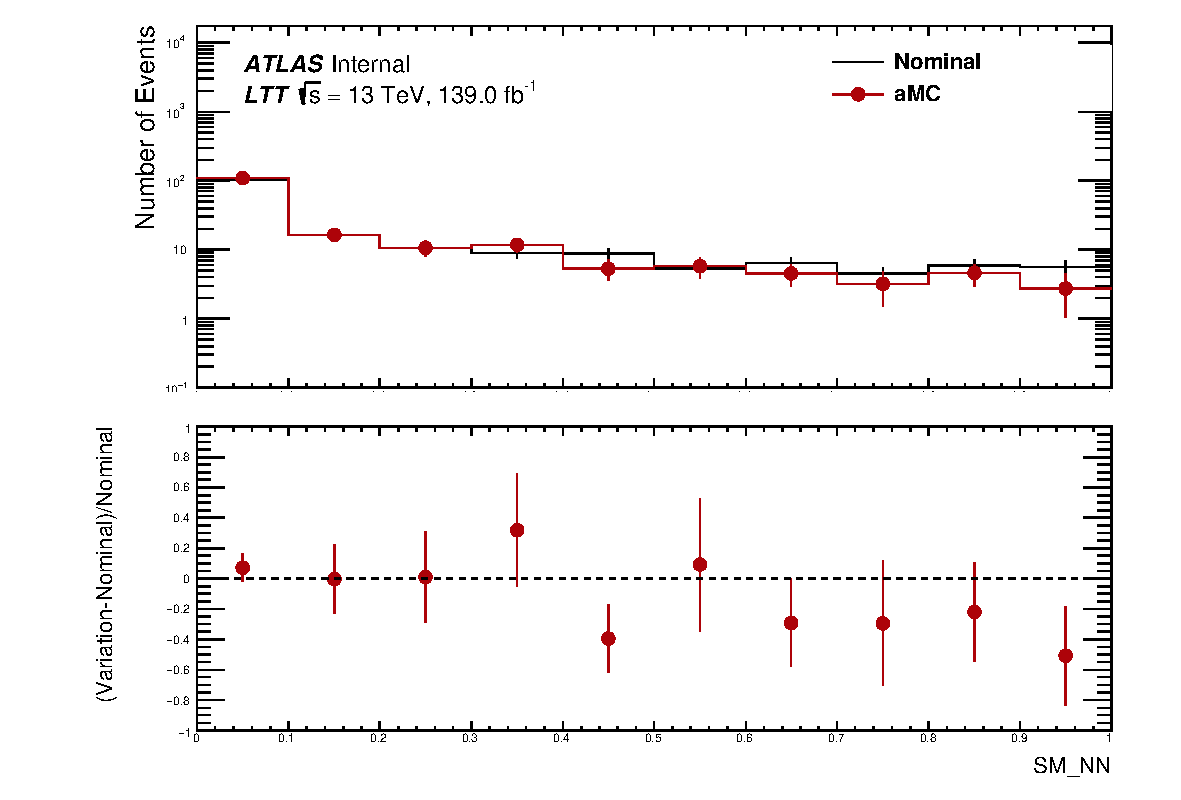
\includegraphics[width=.49\textwidth]{figures/lephad_modelling_systs/LTT/singletop/aMC/Hist_and_ratio_SM_NN_Norm}}
  \subfloat[]{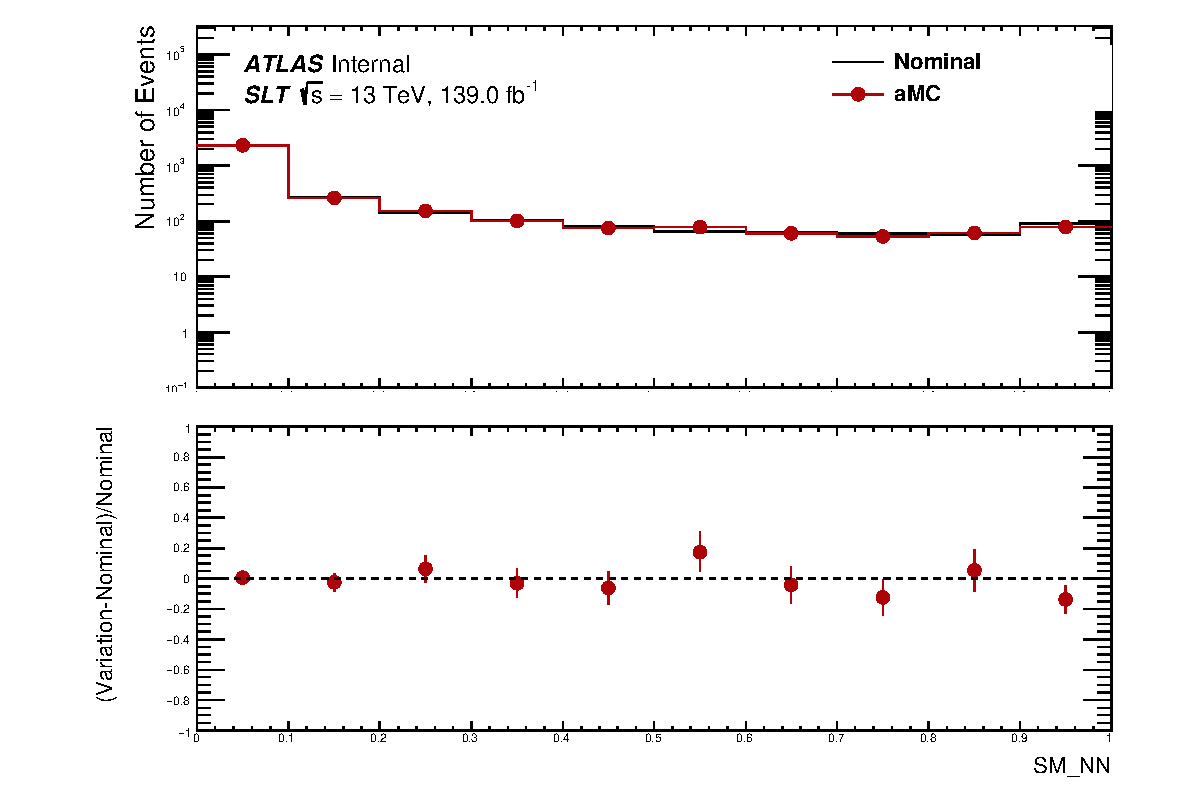
\includegraphics[width=.49\textwidth]{figures/lephad_modelling_systs/SLT/singletop/aMC/Hist_and_ratio_SM_NN_Norm}}
  \caption{LTT (left) and SLT channels (right): shape only SM NN score of the aMC uncertainty .}
  \label{fig:singletopsyst_lephad_aMC_NN}
  \end{figure}


  \begin{figure}
    \centering
    \subfloat[]{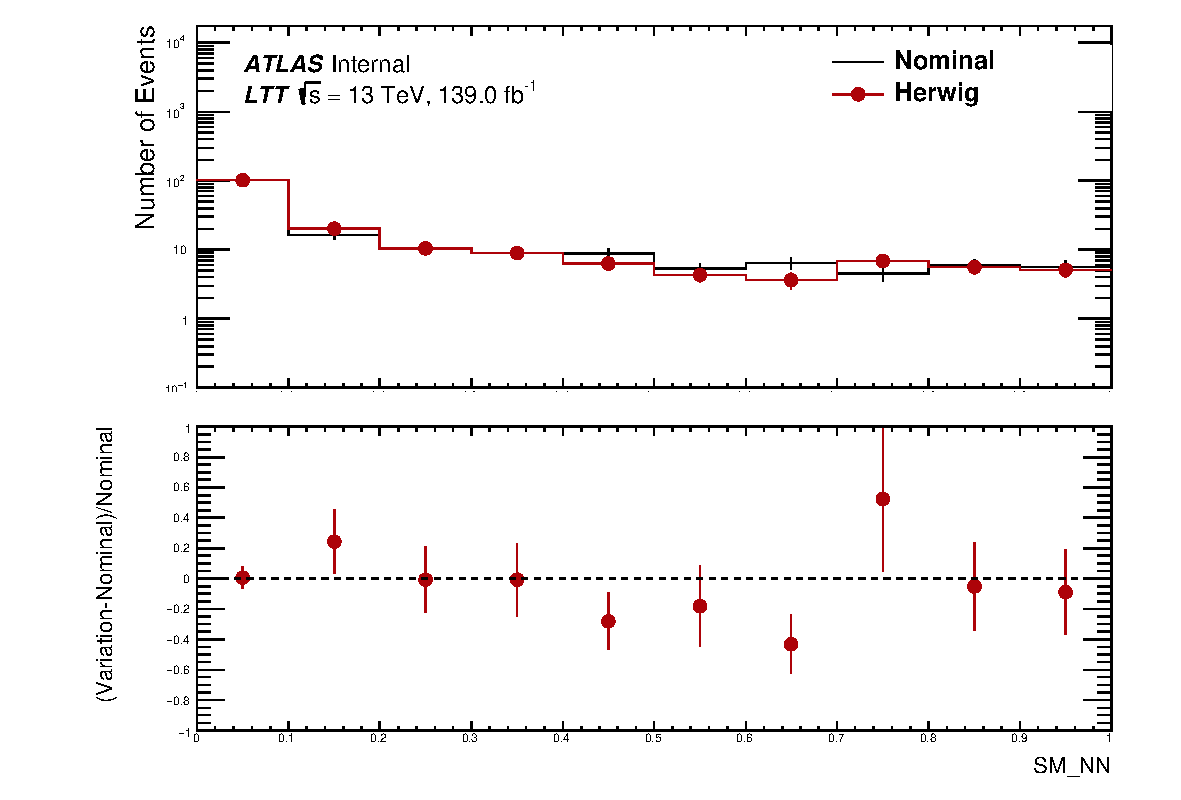
\includegraphics[width=.49\textwidth]{figures/lephad_modelling_systs/LTT/singletop/Herwig/Hist_and_ratio_SM_NN_Norm}}
    \subfloat[]{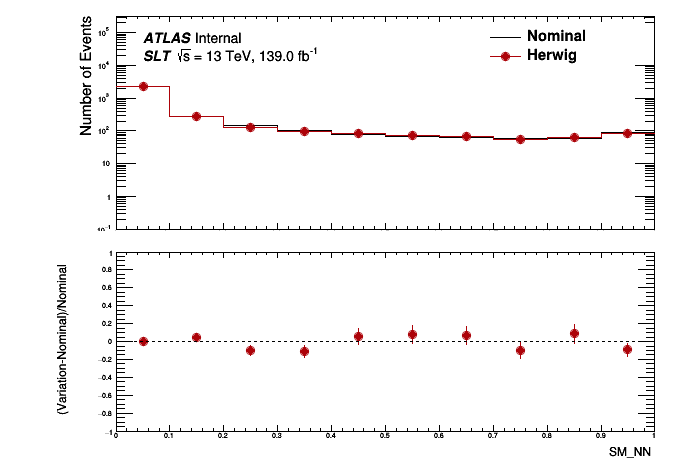
\includegraphics[width=.49\textwidth]{figures/lephad_modelling_systs/SLT/singletop/Herwig/Hist_and_ratio_SM_NN_Norm}}
    \caption{LTT (left) and SLT channels (right): shape only SM NN score of the Herwig uncertainty .}
    \label{fig:singletopsyst_lephad_herwig_NN}
    \end{figure}


\begin{figure}
\centering
\subfloat[]{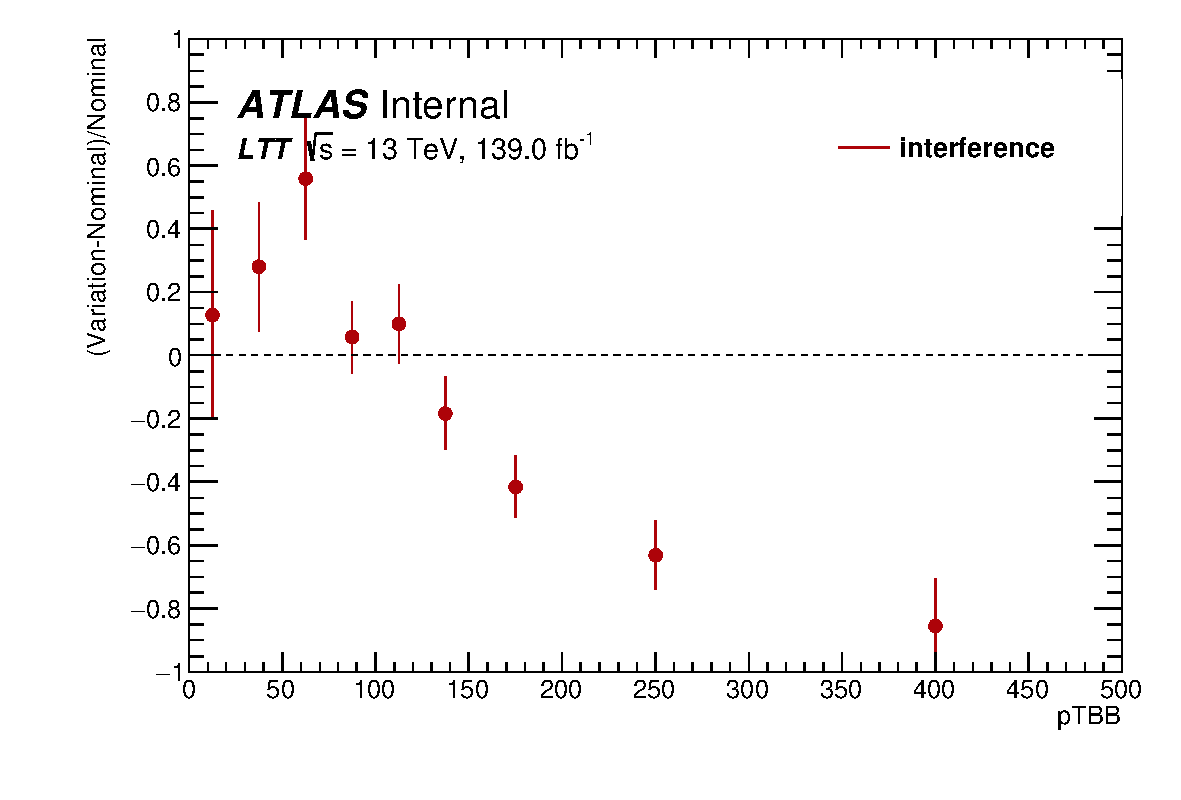
\includegraphics[width=.49\textwidth]{figures/lephad_modelling_systs/LTT/singletop/interference/pTBB_Norm}}
\subfloat[]{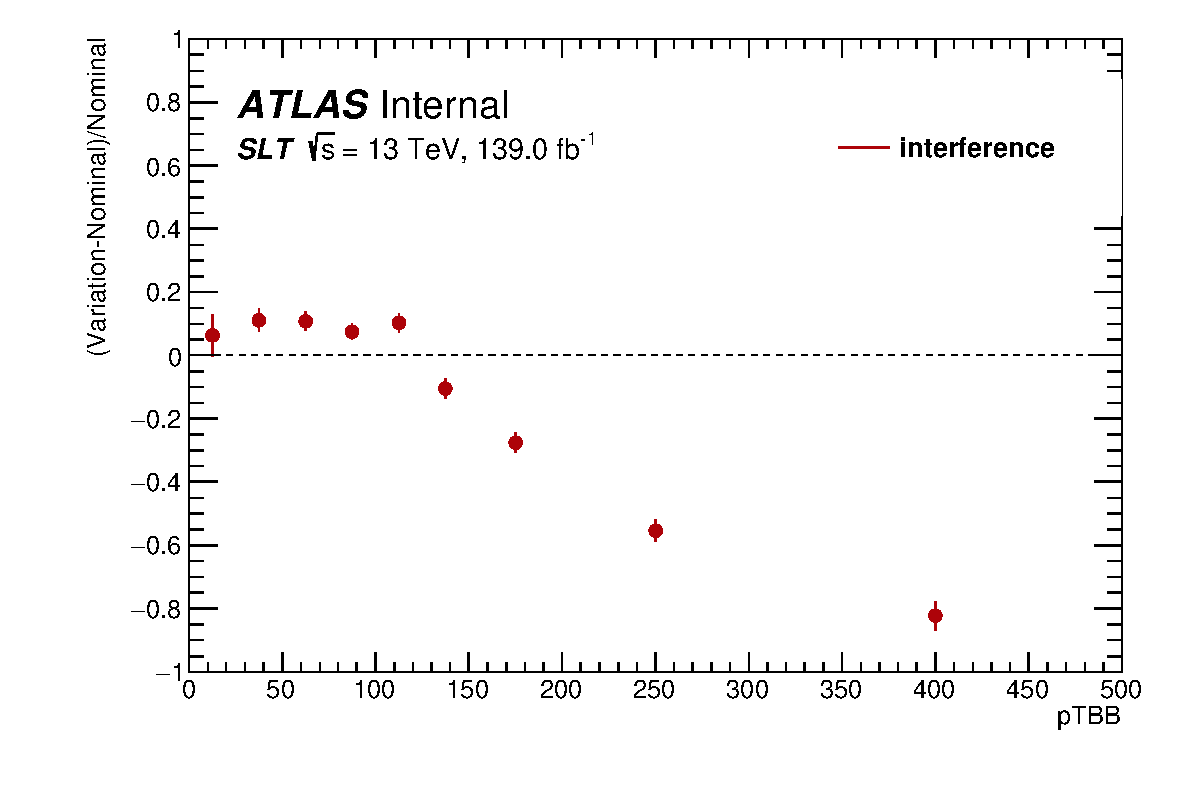
\includegraphics[width=.49\textwidth]{figures/lephad_modelling_systs/SLT/singletop/interference/pTBB_Norm}}
\caption{LTT (left) and SLT channels (right): shape only Parametrisation in bins of $p_T^{bb}$ distribution for $Wt$ DS/DR interference uncertainty.}
\label{fig:singletopsyst_lephad_interference_pTBB}
\end{figure}

\begin{figure}
  \centering
  \subfloat[]{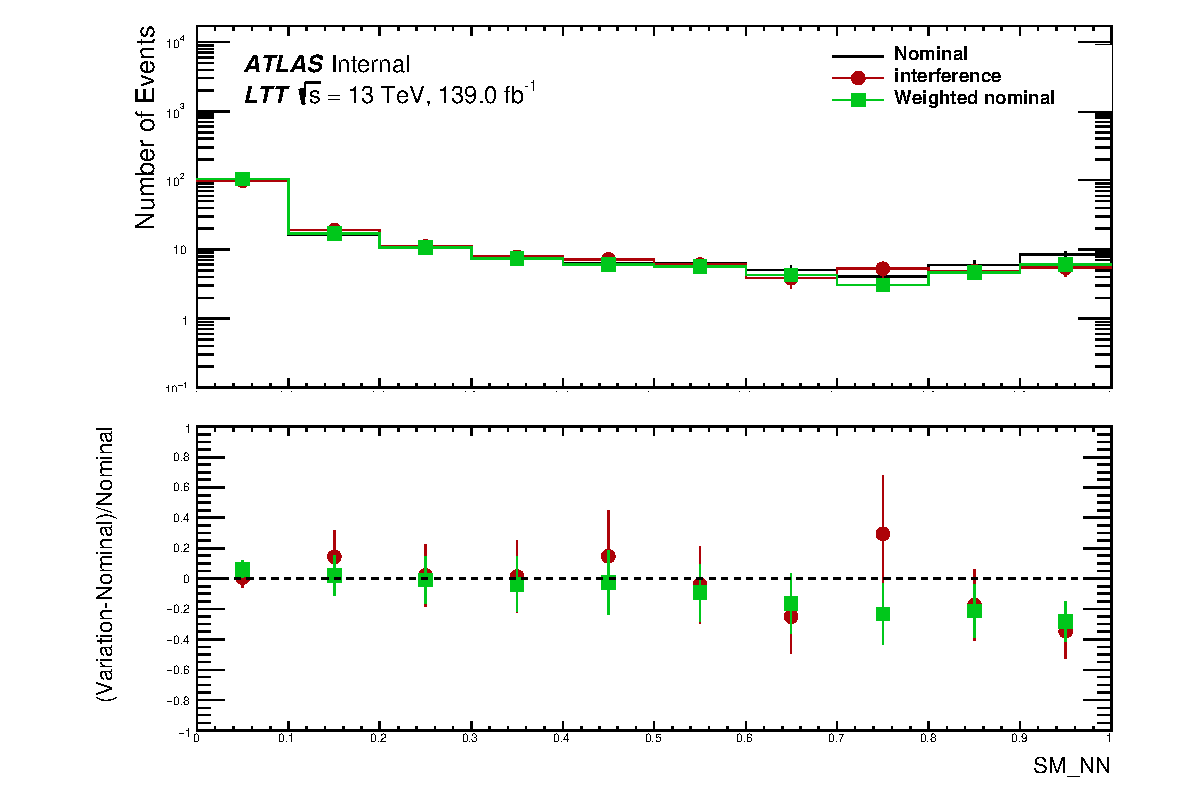
\includegraphics[width=.49\textwidth]{figures/lephad_modelling_systs/LTT/singletop/interference/Hist_and_ratio_SM_NN_Norm}}
  \subfloat[]{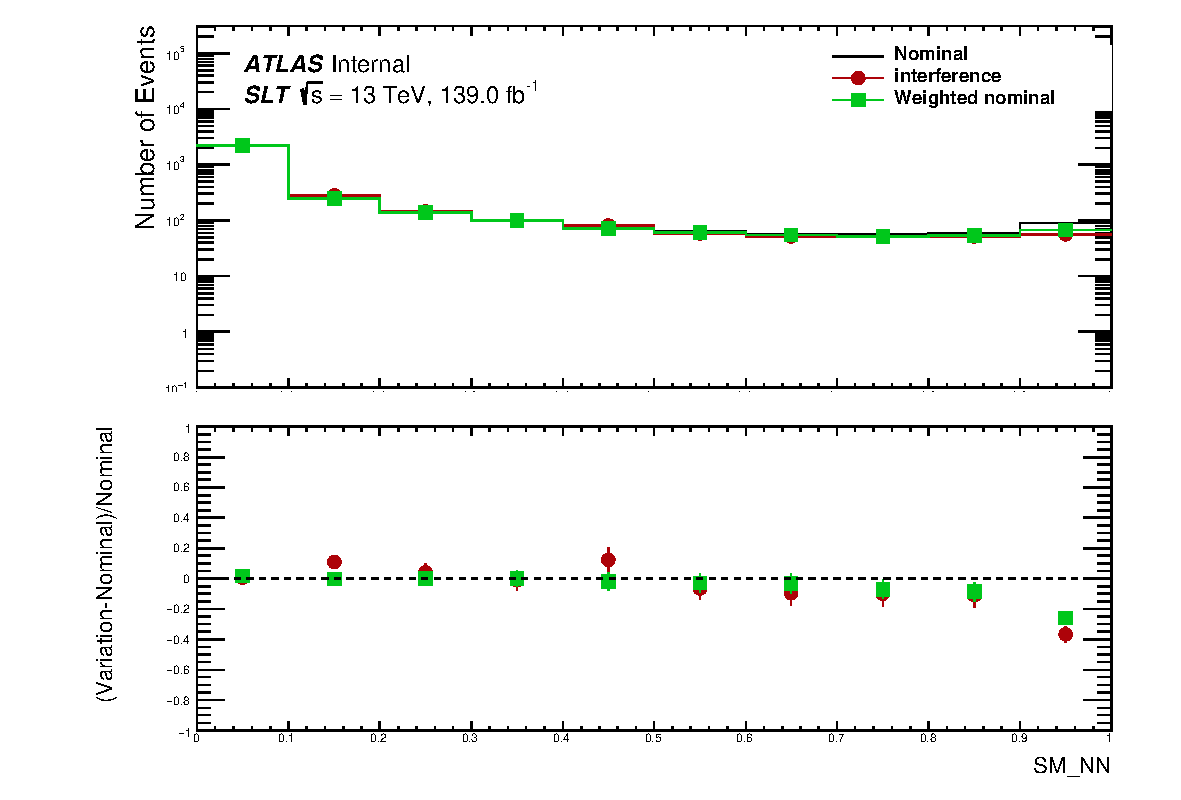
\includegraphics[width=.49\textwidth]{figures/lephad_modelling_systs/SLT/singletop/interference/Hist_and_ratio_SM_NN_Norm}}
  \caption{LTT (left) and SLT channels (right): shape only SM NN score of the $Wt$ DS/DR interference uncertainty .}
  \label{fig:singletopsyst_lephad_interference_NN}
  \end{figure}


\paragraph{Uncertainties on single-top background in the \hadhad channel}\mbox{}\\

The contribution in single-top is even smaller in the \hadhad channel. 
The uncertainties are derived the same way as \lephad channel.
For the uncertainties related to ME, PS, ISR, FSR and PDF variations, only normalisation effect is considered, as summarised in Table~\ref{sec:systs:tab:systematics_normalisations_singletop}. 
For the top interference uncertainty, similar as \lephad channel, the variation (shape+norm.) is parametrised in bins of $p_T^{bb}$, as shown in the ratio plot of Fig.~\ref{fig:singletopsyst_hadhad_interference_pTBB}. Closure of the parametrisation is checked in various BDT/PNN distributions. Good performance is achieved, which can be seem from~\ref{fig:singletopsyst_hadhad_interference_MVA}.
More details about the impact of each variation on the BDT/PNN score distribution can be found in \ref{subsec:appendix_systs_singletop}.

\begin{figure}
  \centering
  \caption{Parametrisation in bins of $p_T^{bb}$ distribution for top interference uncertainty on single-top Wt-channel for \hadhad.}
  \label{fig:singletopsyst_hadhad_interference_pTBB}
\end{figure}

\begin{figure}
  \centering
  \subfloat[]{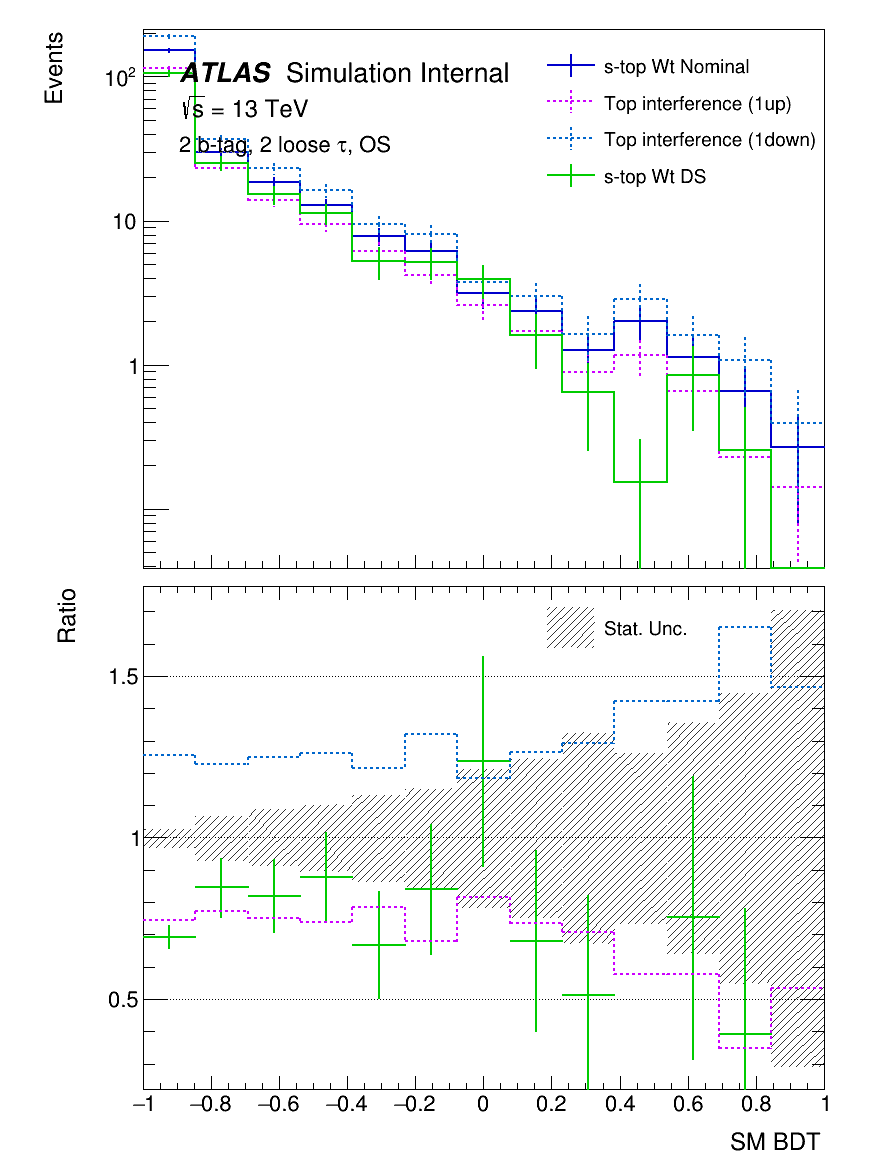
\includegraphics[width=.245\textwidth]{figures/systs/hadhad_stop/2tag2pjet_0ptv_LL_OS_SMBDT_Wt_DS_BDT}}
  \subfloat[]{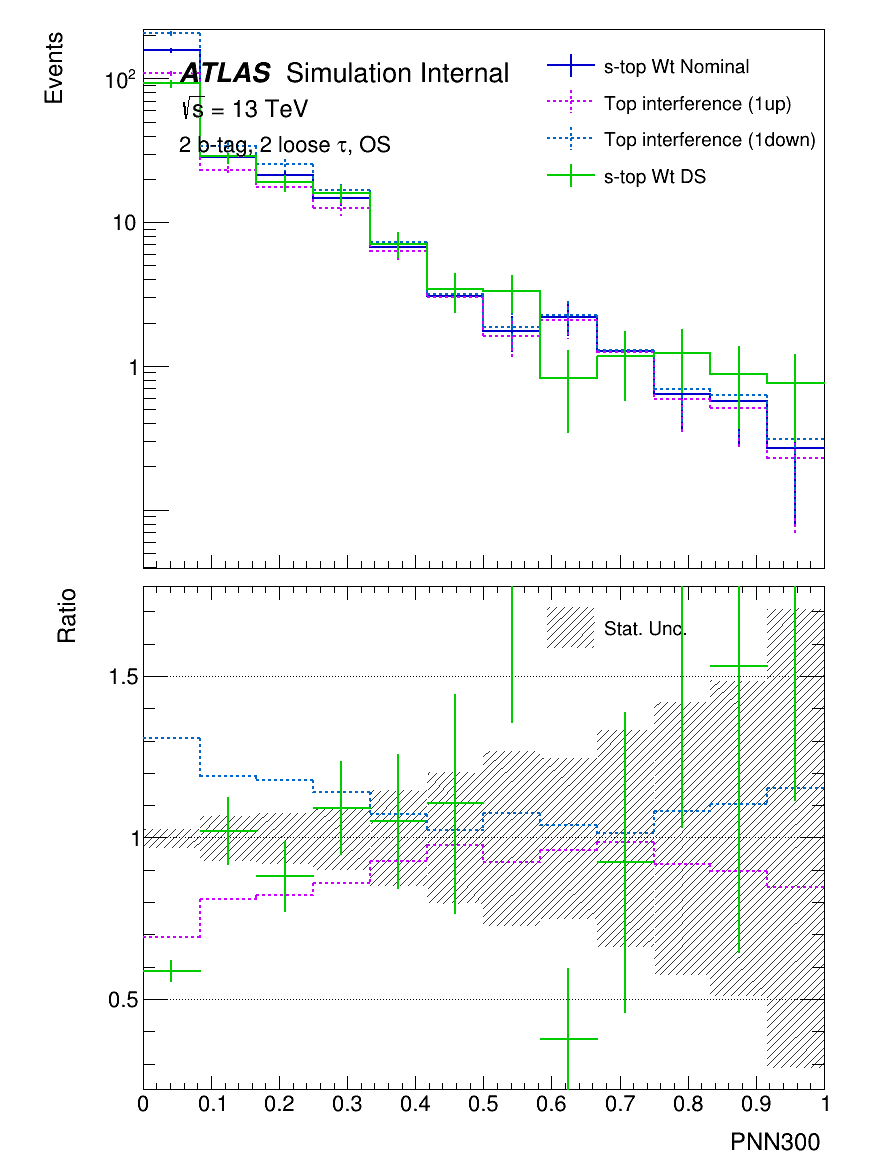
\includegraphics[width=.245\textwidth]{figures/systs/hadhad_stop/2tag2pjet_0ptv_LL_OS_PNN300_Wt_DS_PNN}}
  \subfloat[]{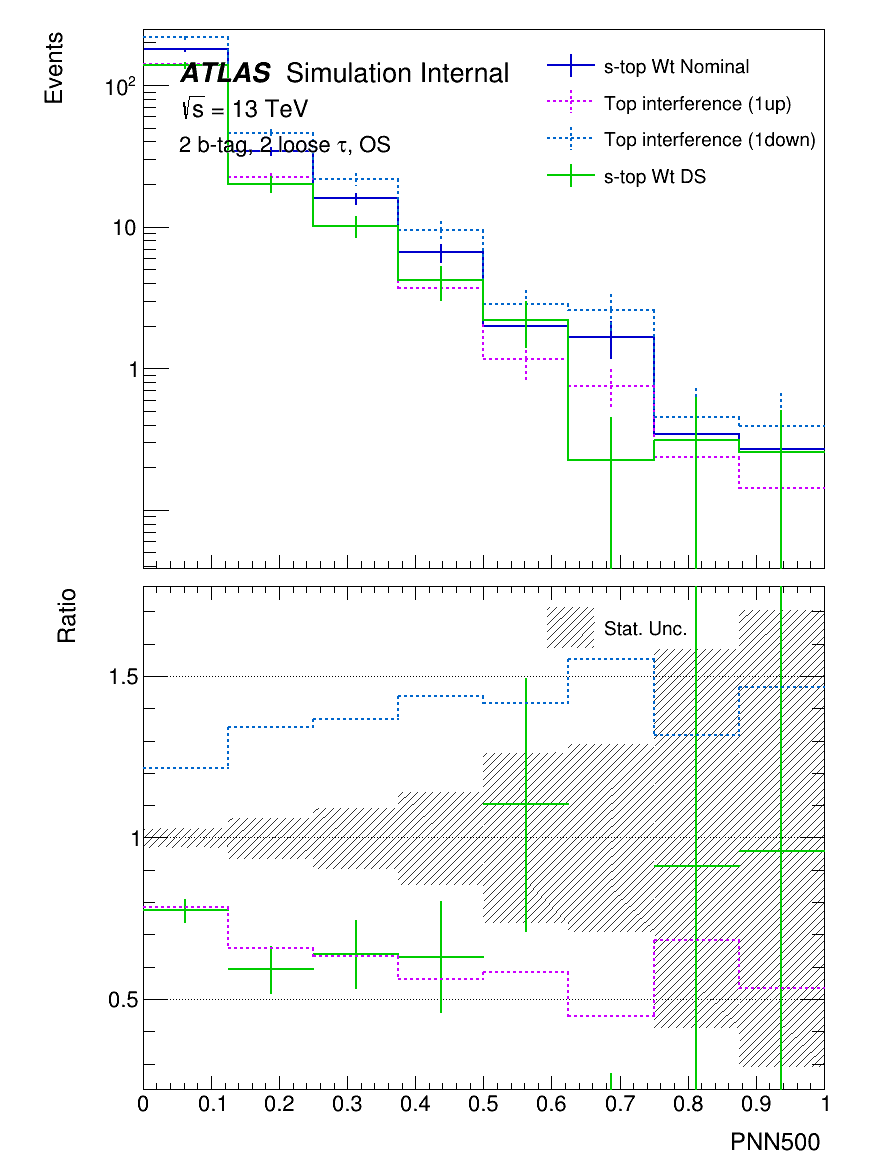
\includegraphics[width=.245\textwidth]{figures/systs/hadhad_stop/2tag2pjet_0ptv_LL_OS_PNN500_Wt_DS_PNN}}
  \subfloat[]{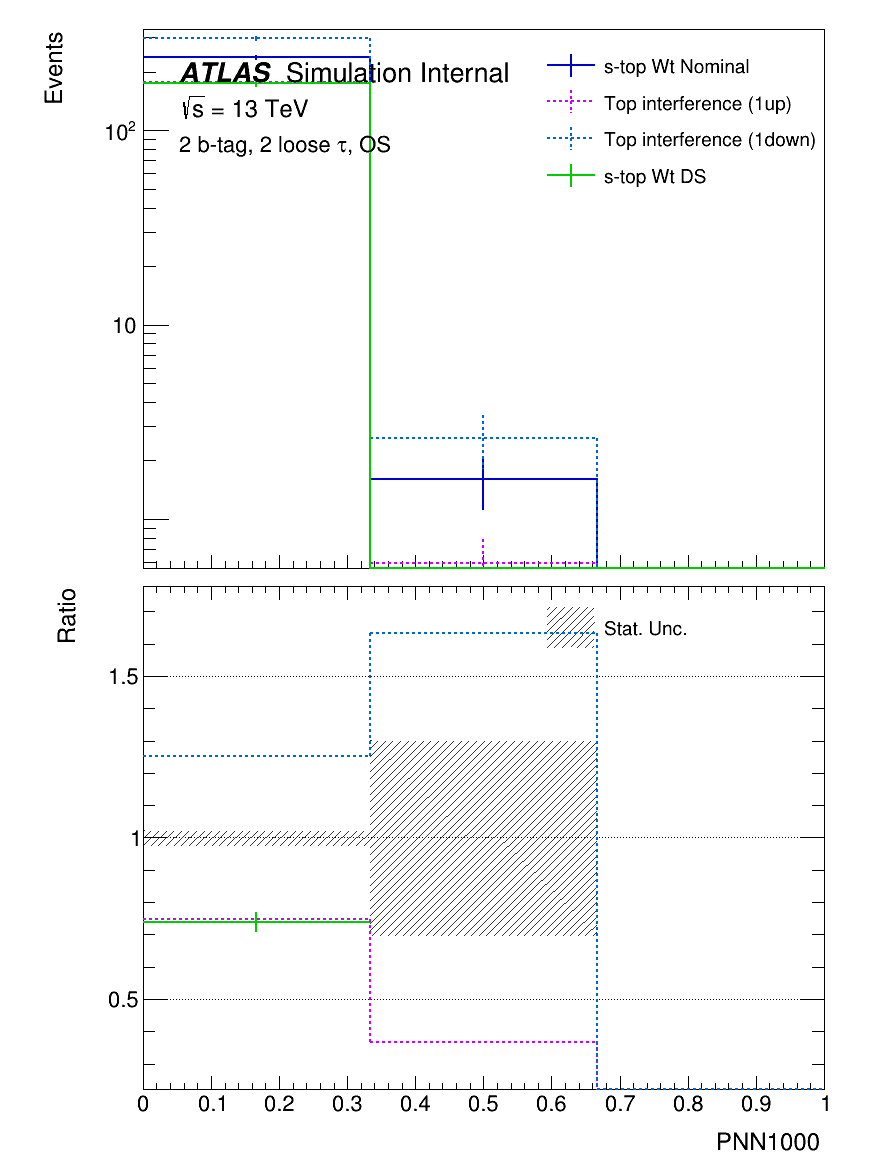
\includegraphics[width=.245\textwidth]{figures/systs/hadhad_stop/2tag2pjet_0ptv_LL_OS_PNN1000_Wt_DS_PNN}}
  \caption{Top interference uncertainty on single-top Wt-channel for \hadhad, in different BDT and PNN distributions.}
  \label{fig:singletopsyst_hadhad_interference_MVA}
\end{figure}

%\begin{table}
%  \centering
%  \small
%  \begin{tabular}{|c|c|}
%  \hline
%  Source & Size in HadHad SR \\
%  \hline
%  ME & $\pm 4.9\%$  \\
%  PS & $\pm 16\%$  \\
%  Single top interference & $\pm 27\%$ \\
%  ISR & $+6.6\%, -4.9\%$ \\
%  FSR & $+8.7\%, -9.4\%$ \\
%  PDF & $+3.2\%, -3.2\%$ \\
%  Total & $\pm 33\%$  \\
%  \hline
%  \end{tabular}
%  \caption{Normalisation acceptance uncertainties for single-top background for the $HH$ \hadhad analysis.}
%  \label{sec:systs:tab:systematics_normalisations_singletop_hadhad}
%\end{table}
  
